\documentclass[1p]{elsarticle_modified}
%\bibliographystyle{elsarticle-num}

%\usepackage[colorlinks]{hyperref}
%\usepackage{abbrmath_seonhwa} %\Abb, \Ascr, \Acal ,\Abf, \Afrak
\usepackage{amsfonts}
\usepackage{amssymb}
\usepackage{amsmath}
\usepackage{amsthm}
\usepackage{scalefnt}
\usepackage{amsbsy}
\usepackage{kotex}
\usepackage{caption}
\usepackage{subfig}
\usepackage{color}
\usepackage{graphicx}
\usepackage{xcolor} %% white, black, red, green, blue, cyan, magenta, yellow
\usepackage{float}
\usepackage{setspace}
\usepackage{hyperref}

\usepackage{tikz}
\usetikzlibrary{arrows}

\usepackage{multirow}
\usepackage{array} % fixed length table
\usepackage{hhline}

%%%%%%%%%%%%%%%%%%%%%
\makeatletter
\renewcommand*\env@matrix[1][\arraystretch]{%
	\edef\arraystretch{#1}%
	\hskip -\arraycolsep
	\let\@ifnextchar\new@ifnextchar
	\array{*\c@MaxMatrixCols c}}
\makeatother %https://tex.stackexchange.com/questions/14071/how-can-i-increase-the-line-spacing-in-a-matrix
%%%%%%%%%%%%%%%

\usepackage[normalem]{ulem}

\newcommand{\msout}[1]{\ifmmode\text{\sout{\ensuremath{#1}}}\else\sout{#1}\fi}
%SOURCE: \msout is \stkout macro in https://tex.stackexchange.com/questions/20609/strikeout-in-math-mode

\newcommand{\cancel}[1]{
	\ifmmode
	{\color{red}\msout{#1}}
	\else
	{\color{red}\sout{#1}}
	\fi
}

\newcommand{\add}[1]{
	{\color{blue}\uwave{#1}}
}

\newcommand{\replace}[2]{
	\ifmmode
	{\color{red}\msout{#1}}{\color{blue}\uwave{#2}}
	\else
	{\color{red}\sout{#1}}{\color{blue}\uwave{#2}}
	\fi
}

\newcommand{\Sol}{\mathcal{S}} %segment
\newcommand{\D}{D} %diagram
\newcommand{\A}{\mathcal{A}} %arc


%%%%%%%%%%%%%%%%%%%%%%%%%%%%%5 test

\def\sl{\operatorname{\textup{SL}}(2,\Cbb)}
\def\psl{\operatorname{\textup{PSL}}(2,\Cbb)}
\def\quan{\mkern 1mu \triangleright \mkern 1mu}

\theoremstyle{definition}
\newtheorem{thm}{Theorem}[section]
\newtheorem{prop}[thm]{Proposition}
\newtheorem{lem}[thm]{Lemma}
\newtheorem{ques}[thm]{Question}
\newtheorem{cor}[thm]{Corollary}
\newtheorem{defn}[thm]{Definition}
\newtheorem{exam}[thm]{Example}
\newtheorem{rmk}[thm]{Remark}
\newtheorem{alg}[thm]{Algorithm}

\newcommand{\I}{\sqrt{-1}}
\begin{document}

%\begin{frontmatter}
%
%\title{Boundary parabolic representations of knots up to 8 crossings}
%
%%% Group authors per affiliation:
%\author{Yunhi Cho} 
%\address{Department of Mathematics, University of Seoul, Seoul, Korea}
%\ead{yhcho@uos.ac.kr}
%
%
%\author{Seonhwa Kim} %\fnref{s_kim}}
%\address{Center for Geometry and Physics, Institute for Basic Science, Pohang, 37673, Korea}
%\ead{ryeona17@ibs.re.kr}
%
%\author{Hyuk Kim}
%\address{Department of Mathematical Sciences, Seoul National University, Seoul 08826, Korea}
%\ead{hyukkim@snu.ac.kr}
%
%\author{Seokbeom Yoon}
%\address{Department of Mathematical Sciences, Seoul National University, Seoul, 08826,  Korea}
%\ead{sbyoon15@snu.ac.kr}
%
%\begin{abstract}
%We find all boundary parabolic representation of knots up to 8 crossings.
%
%\end{abstract}
%\begin{keyword}
%    \MSC[2010] 57M25 
%\end{keyword}
%
%\end{frontmatter}

%\linenumbers
%\tableofcontents
%
\newcommand\colored[1]{\textcolor{white}{\rule[-0.35ex]{0.8em}{1.4ex}}\kern-0.8em\color{red} #1}%
%\newcommand\colored[1]{\textcolor{white}{ #1}\kern-2.17ex	\textcolor{white}{ #1}\kern-1.81ex	\textcolor{white}{ #1}\kern-2.15ex\color{red}#1	}

{\Large $\underline{12a_{0267}~(K12a_{0267})}$}

\setlength{\tabcolsep}{10pt}
\renewcommand{\arraystretch}{1.6}
\vspace{1cm}\begin{tabular}{m{100pt}>{\centering\arraybackslash}m{274pt}}
\multirow{5}{120pt}{
	\centering
	\includegraphics[width=112pt]{../../../GIT/diagram.site/Diagrams/png/1068_12a_0267.png}\\
\ \ \ A knot diagram\footnotemark}&
\allowdisplaybreaks
\textbf{Linearized knot diagam} \\
\cline{2-2}
 &
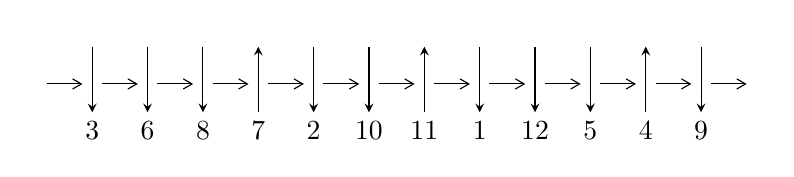
\begin{tikzpicture}[x=20pt, y=17pt]
	% nodes
	\node (C0) at (0, 0) {};
	\node (C1) at (1, 0) {};
	\node (C1U) at (1, +1) {};
	\node (C1D) at (1, -1) {3};

	\node (C2) at (2, 0) {};
	\node (C2U) at (2, +1) {};
	\node (C2D) at (2, -1) {6};

	\node (C3) at (3, 0) {};
	\node (C3U) at (3, +1) {};
	\node (C3D) at (3, -1) {8};

	\node (C4) at (4, 0) {};
	\node (C4U) at (4, +1) {};
	\node (C4D) at (4, -1) {7};

	\node (C5) at (5, 0) {};
	\node (C5U) at (5, +1) {};
	\node (C5D) at (5, -1) {2};

	\node (C6) at (6, 0) {};
	\node (C6U) at (6, +1) {};
	\node (C6D) at (6, -1) {10};

	\node (C7) at (7, 0) {};
	\node (C7U) at (7, +1) {};
	\node (C7D) at (7, -1) {11};

	\node (C8) at (8, 0) {};
	\node (C8U) at (8, +1) {};
	\node (C8D) at (8, -1) {1};

	\node (C9) at (9, 0) {};
	\node (C9U) at (9, +1) {};
	\node (C9D) at (9, -1) {12};

	\node (C10) at (10, 0) {};
	\node (C10U) at (10, +1) {};
	\node (C10D) at (10, -1) {5};

	\node (C11) at (11, 0) {};
	\node (C11U) at (11, +1) {};
	\node (C11D) at (11, -1) {4};

	\node (C12) at (12, 0) {};
	\node (C12U) at (12, +1) {};
	\node (C12D) at (12, -1) {9};
	\node (C13) at (13, 0) {};

	% arrows
	\draw[->,>={angle 60}]
	(C0) edge (C1) (C1) edge (C2) (C2) edge (C3) (C3) edge (C4) (C4) edge (C5) (C5) edge (C6) (C6) edge (C7) (C7) edge (C8) (C8) edge (C9) (C9) edge (C10) (C10) edge (C11) (C11) edge (C12) (C12) edge (C13) ;	\draw[->,>=stealth]
	(C1U) edge (C1D) (C2U) edge (C2D) (C3U) edge (C3D) (C4D) edge (C4U) (C5U) edge (C5D) (C6U) edge (C6D) (C7D) edge (C7U) (C8U) edge (C8D) (C9U) edge (C9D) (C10U) edge (C10D) (C11D) edge (C11U) (C12U) edge (C12D) ;
	\end{tikzpicture} \\
\hhline{~~} \\& 
\textbf{Solving Sequence} \\ \cline{2-2} 
 &
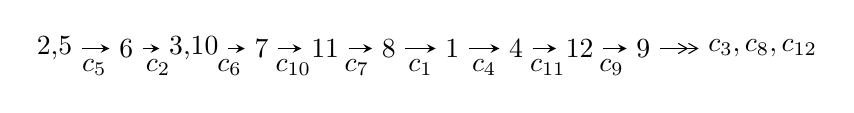
\begin{tikzpicture}[x=23pt, y=7pt]
	% node
	\node (A0) at (-1/8, 0) {2,5};
	\node (A1) at (1, 0) {6};
	\node (A2) at (33/16, 0) {3,10};
	\node (A3) at (25/8, 0) {7};
	\node (A4) at (33/8, 0) {11};
	\node (A5) at (41/8, 0) {8};
	\node (A6) at (49/8, 0) {1};
	\node (A7) at (57/8, 0) {4};
	\node (A8) at (65/8, 0) {12};
	\node (A9) at (73/8, 0) {9};
	\node (C1) at (1/2, -1) {$c_{5}$};
	\node (C2) at (3/2, -1) {$c_{2}$};
	\node (C3) at (21/8, -1) {$c_{6}$};
	\node (C4) at (29/8, -1) {$c_{10}$};
	\node (C5) at (37/8, -1) {$c_{7}$};
	\node (C6) at (45/8, -1) {$c_{1}$};
	\node (C7) at (53/8, -1) {$c_{4}$};
	\node (C8) at (61/8, -1) {$c_{11}$};
	\node (C9) at (69/8, -1) {$c_{9}$};
	\node (A10) at (11, 0) {$c_{3},c_{8},c_{12}$};

	% edge
	\draw[->,>=stealth]	
	(A0) edge (A1) (A1) edge (A2) (A2) edge (A3) (A3) edge (A4) (A4) edge (A5) (A5) edge (A6) (A6) edge (A7) (A7) edge (A8) (A8) edge (A9) ;
	\draw[->>,>={angle 60}]	
	(A9) edge (A10);
\end{tikzpicture} \\ 

\end{tabular} \\

\footnotetext{
The image of knot diagram is generated by the software ``\textbf{Draw programme}" developed by Andrew Bartholomew(\url{http://www.layer8.co.uk/maths/draw/index.htm\#Running-draw}), where we modified some parts for our purpose(\url{https://github.com/CATsTAILs/LinksPainter}).
}\phantom \\ \newline 
\centering \textbf{Ideals for irreducible components\footnotemark of $X_{\text{par}}$} 
 
\begin{align*}
I^u_{1}&=\langle 
2.48175\times10^{423} u^{145}+6.47417\times10^{423} u^{144}+\cdots+2.60431\times10^{425} b-4.75085\times10^{426},\\
\phantom{I^u_{1}}&\phantom{= \langle  }1.32031\times10^{428} u^{145}+5.69757\times10^{428} u^{144}+\cdots+7.55251\times10^{427} a-5.42178\times10^{430},\\
\phantom{I^u_{1}}&\phantom{= \langle  }u^{146}+4 u^{145}+\cdots-333 u+145\rangle \\
I^u_{2}&=\langle 
-22 u^{28}+63 u^{27}+\cdots+b+40,\;23 u^{28}-38 u^{27}+\cdots+a-9,\;u^{29}-3 u^{28}+\cdots-3 u+1\rangle \\
I^u_{3}&=\langle 
-8 a^5+5 a^4+4 a^3-31 a^2+69 b-64 a+78,\;a^6-2 a^5+6 a^3-2 a^2-15 a+17,\;u+1\rangle \\
\\
\end{align*}
\raggedright * 3 irreducible components of $\dim_{\mathbb{C}}=0$, with total 181 representations.\\
\footnotetext{All coefficients of polynomials are rational numbers. But the coefficients are sometimes approximated in decimal forms when there is not enough margin.}
\newpage
\renewcommand{\arraystretch}{1}
\centering \section*{I. $I^u_{1}= \langle 2.48\times10^{423} u^{145}+6.47\times10^{423} u^{144}+\cdots+2.60\times10^{425} b-4.75\times10^{426},\;1.32\times10^{428} u^{145}+5.70\times10^{428} u^{144}+\cdots+7.55\times10^{427} a-5.42\times10^{430},\;u^{146}+4 u^{145}+\cdots-333 u+145 \rangle$}
\flushleft \textbf{(i) Arc colorings}\\
\begin{tabular}{m{7pt} m{180pt} m{7pt} m{180pt} }
\flushright $a_{2}=$&$\begin{pmatrix}0\\u\end{pmatrix}$ \\
\flushright $a_{5}=$&$\begin{pmatrix}1\\0\end{pmatrix}$ \\
\flushright $a_{6}=$&$\begin{pmatrix}1\\u^2\end{pmatrix}$ \\
\flushright $a_{3}=$&$\begin{pmatrix}- u\\- u^3+u\end{pmatrix}$ \\
\flushright $a_{10}=$&$\begin{pmatrix}-1.74818 u^{145}-7.54395 u^{144}+\cdots+409.136 u+717.878\\-0.00952937 u^{145}-0.0248594 u^{144}+\cdots+17.2071 u+18.2422\end{pmatrix}$ \\
\flushright $a_{7}=$&$\begin{pmatrix}-0.435446 u^{145}-1.88667 u^{144}+\cdots+130.906 u+250.926\\0.114455 u^{145}+0.546935 u^{144}+\cdots+7.79061 u-52.6943\end{pmatrix}$ \\
\flushright $a_{11}=$&$\begin{pmatrix}-1.73865 u^{145}-7.51909 u^{144}+\cdots+391.929 u+699.635\\-0.00952937 u^{145}-0.0248594 u^{144}+\cdots+17.2071 u+18.2422\end{pmatrix}$ \\
\flushright $a_{8}=$&$\begin{pmatrix}1.22486 u^{145}+5.37461 u^{144}+\cdots-224.823 u-480.791\\0.0428686 u^{145}+0.227799 u^{144}+\cdots+11.5021 u-11.9860\end{pmatrix}$ \\
\flushright $a_{1}=$&$\begin{pmatrix}u^3\\u^5- u^3+u\end{pmatrix}$ \\
\flushright $a_{4}=$&$\begin{pmatrix}0.391087 u^{145}+1.84118 u^{144}+\cdots-36.1350 u-159.522\\0.223870 u^{145}+0.982120 u^{144}+\cdots-18.3317 u-65.0821\end{pmatrix}$ \\
\flushright $a_{12}=$&$\begin{pmatrix}0.120587 u^{145}+0.503240 u^{144}+\cdots-24.4200 u-68.1190\\0.120621 u^{145}+0.526531 u^{144}+\cdots-34.8729 u-61.0393\end{pmatrix}$ \\
\flushright $a_{9}=$&$\begin{pmatrix}1.24939 u^{145}+5.50261 u^{144}+\cdots-217.275 u-493.079\\0.194473 u^{145}+0.884878 u^{144}+\cdots-14.3452 u-60.1351\end{pmatrix}$\\&\end{tabular}
\flushleft \textbf{(ii) Obstruction class $= -1$}\\~\\
\flushleft \textbf{(iii) Cusp Shapes $= -0.772054 u^{145}-3.28462 u^{144}+\cdots-30.4527 u+140.299$}\\~\\
\newpage\renewcommand{\arraystretch}{1}
\flushleft \textbf{(iv) u-Polynomials at the component}\newline \\
\begin{tabular}{m{50pt}|m{274pt}}
Crossings & \hspace{64pt}u-Polynomials at each crossing \\
\hline $$\begin{aligned}c_{1}\end{aligned}$$&$\begin{aligned}
&u^{146}+56 u^{145}+\cdots+723369 u+21025
\end{aligned}$\\
\hline $$\begin{aligned}c_{2},c_{5}\end{aligned}$$&$\begin{aligned}
&u^{146}+4 u^{145}+\cdots-333 u+145
\end{aligned}$\\
\hline $$\begin{aligned}c_{3}\end{aligned}$$&$\begin{aligned}
&u^{146}+4 u^{145}+\cdots+2468988890 u+899654983
\end{aligned}$\\
\hline $$\begin{aligned}c_{4}\end{aligned}$$&$\begin{aligned}
&u^{146}+12 u^{145}+\cdots+18 u+1
\end{aligned}$\\
\hline $$\begin{aligned}c_{6}\end{aligned}$$&$\begin{aligned}
&u^{146}- u^{145}+\cdots+13382 u-2117
\end{aligned}$\\
\hline $$\begin{aligned}c_{7}\end{aligned}$$&$\begin{aligned}
&u^{146}-4 u^{144}+\cdots+672 u+320
\end{aligned}$\\
\hline $$\begin{aligned}c_{8},c_{9},c_{12}\end{aligned}$$&$\begin{aligned}
&u^{146}+5 u^{145}+\cdots+24 u-1
\end{aligned}$\\
\hline $$\begin{aligned}c_{10}\end{aligned}$$&$\begin{aligned}
&u^{146}- u^{145}+\cdots+1200 u+145
\end{aligned}$\\
\hline $$\begin{aligned}c_{11}\end{aligned}$$&$\begin{aligned}
&u^{146}-5 u^{145}+\cdots-1206 u+145
\end{aligned}$\\
\hline
\end{tabular}\\~\\
\newpage\renewcommand{\arraystretch}{1}
\flushleft \textbf{(v) Riley Polynomials at the component}\newline \\
\begin{tabular}{m{50pt}|m{274pt}}
Crossings & \hspace{64pt}Riley Polynomials at each crossing \\
\hline $$\begin{aligned}c_{1}\end{aligned}$$&$\begin{aligned}
&y^{146}+76 y^{145}+\cdots-56026237661 y+442050625
\end{aligned}$\\
\hline $$\begin{aligned}c_{2},c_{5}\end{aligned}$$&$\begin{aligned}
&y^{146}-56 y^{145}+\cdots-723369 y+21025
\end{aligned}$\\
\hline $$\begin{aligned}c_{3}\end{aligned}$$&$\begin{aligned}
&y^{146}+48 y^{145}+\cdots-8.05\times10^{19} y+8.09\times10^{17}
\end{aligned}$\\
\hline $$\begin{aligned}c_{4}\end{aligned}$$&$\begin{aligned}
&y^{146}+4 y^{145}+\cdots+274 y+1
\end{aligned}$\\
\hline $$\begin{aligned}c_{6}\end{aligned}$$&$\begin{aligned}
&y^{146}+31 y^{145}+\cdots+165806780 y+4481689
\end{aligned}$\\
\hline $$\begin{aligned}c_{7}\end{aligned}$$&$\begin{aligned}
&y^{146}-8 y^{145}+\cdots-3339264 y+102400
\end{aligned}$\\
\hline $$\begin{aligned}c_{8},c_{9},c_{12}\end{aligned}$$&$\begin{aligned}
&y^{146}+147 y^{145}+\cdots+14 y+1
\end{aligned}$\\
\hline $$\begin{aligned}c_{10}\end{aligned}$$&$\begin{aligned}
&y^{146}+17 y^{145}+\cdots+1475950 y+21025
\end{aligned}$\\
\hline $$\begin{aligned}c_{11}\end{aligned}$$&$\begin{aligned}
&y^{146}-7 y^{145}+\cdots-324306 y+21025
\end{aligned}$\\
\hline
\end{tabular}\\~\\
\newpage\flushleft \textbf{(vi) Complex Volumes and Cusp Shapes}
$$\begin{array}{c|c|c}  
\text{Solutions to }I^u_{1}& \I (\text{vol} + \sqrt{-1}CS) & \text{Cusp shape}\\
 \hline 
\begin{aligned}
u &= -0.717312 + 0.699409 I \\
a &= -2.34714 - 1.26596 I \\
b &= -0.079322 + 0.544577 I\end{aligned}
 & \phantom{-}9.86898 - 3.45452 I & \phantom{-0.000000 } 0 \\ \hline\begin{aligned}
u &= -0.717312 - 0.699409 I \\
a &= -2.34714 + 1.26596 I \\
b &= -0.079322 - 0.544577 I\end{aligned}
 & \phantom{-}9.86898 + 3.45452 I & \phantom{-0.000000 } 0 \\ \hline\begin{aligned}
u &= \phantom{-}0.751663 + 0.666797 I \\
a &= -0.724199 - 0.469522 I \\
b &= -0.572940 + 1.018600 I\end{aligned}
 & \phantom{-}4.66153 + 3.56872 I & \phantom{-0.000000 } 0 \\ \hline\begin{aligned}
u &= \phantom{-}0.751663 - 0.666797 I \\
a &= -0.724199 + 0.469522 I \\
b &= -0.572940 - 1.018600 I\end{aligned}
 & \phantom{-}4.66153 - 3.56872 I & \phantom{-0.000000 } 0 \\ \hline\begin{aligned}
u &= \phantom{-}1.002600 + 0.195131 I \\
a &= \phantom{-}2.13983 + 0.28539 I \\
b &= \phantom{-}0.482851 + 0.453150 I\end{aligned}
 & \phantom{-}0.85295 - 5.12362 I & \phantom{-0.000000 } 0 \\ \hline\begin{aligned}
u &= \phantom{-}1.002600 - 0.195131 I \\
a &= \phantom{-}2.13983 - 0.28539 I \\
b &= \phantom{-}0.482851 - 0.453150 I\end{aligned}
 & \phantom{-}0.85295 + 5.12362 I & \phantom{-0.000000 } 0 \\ \hline\begin{aligned}
u &= \phantom{-}0.783873 + 0.582905 I \\
a &= -0.71241 + 2.00247 I \\
b &= -1.98372 + 0.05552 I\end{aligned}
 & -0.191919 + 0.970948 I & \phantom{-0.000000 } 0 \\ \hline\begin{aligned}
u &= \phantom{-}0.783873 - 0.582905 I \\
a &= -0.71241 - 2.00247 I \\
b &= -1.98372 - 0.05552 I\end{aligned}
 & -0.191919 - 0.970948 I & \phantom{-0.000000 } 0 \\ \hline\begin{aligned}
u &= -0.723954 + 0.736563 I \\
a &= -0.170958 + 0.108878 I \\
b &= \phantom{-}0.89695 + 1.32014 I\end{aligned}
 & \phantom{-}3.10050 - 3.62856 I & \phantom{-0.000000 } 0 \\ \hline\begin{aligned}
u &= -0.723954 - 0.736563 I \\
a &= -0.170958 - 0.108878 I \\
b &= \phantom{-}0.89695 - 1.32014 I\end{aligned}
 & \phantom{-}3.10050 + 3.62856 I & \phantom{-0.000000 } 0\\
 \hline 
 \end{array}$$\newpage$$\begin{array}{c|c|c}  
\text{Solutions to }I^u_{1}& \I (\text{vol} + \sqrt{-1}CS) & \text{Cusp shape}\\
 \hline 
\begin{aligned}
u &= -0.797875 + 0.656098 I \\
a &= \phantom{-}1.167590 + 0.442098 I \\
b &= \phantom{-}0.972968 + 0.380891 I\end{aligned}
 & \phantom{-}0.107696 - 0.580505 I & \phantom{-0.000000 } 0 \\ \hline\begin{aligned}
u &= -0.797875 - 0.656098 I \\
a &= \phantom{-}1.167590 - 0.442098 I \\
b &= \phantom{-}0.972968 - 0.380891 I\end{aligned}
 & \phantom{-}0.107696 + 0.580505 I & \phantom{-0.000000 } 0 \\ \hline\begin{aligned}
u &= \phantom{-}0.583336 + 0.856509 I \\
a &= \phantom{-}0.174856 + 0.109704 I \\
b &= \phantom{-}0.083596 - 0.849372 I\end{aligned}
 & \phantom{-}4.28577 + 1.52049 I & \phantom{-0.000000 } 0 \\ \hline\begin{aligned}
u &= \phantom{-}0.583336 - 0.856509 I \\
a &= \phantom{-}0.174856 - 0.109704 I \\
b &= \phantom{-}0.083596 + 0.849372 I\end{aligned}
 & \phantom{-}4.28577 - 1.52049 I & \phantom{-0.000000 } 0 \\ \hline\begin{aligned}
u &= -1.027870 + 0.186062 I \\
a &= \phantom{-}2.17640 - 0.35403 I \\
b &= \phantom{-}1.40942 - 1.24508 I\end{aligned}
 & -3.22736 - 0.23964 I & \phantom{-0.000000 } 0 \\ \hline\begin{aligned}
u &= -1.027870 - 0.186062 I \\
a &= \phantom{-}2.17640 + 0.35403 I \\
b &= \phantom{-}1.40942 + 1.24508 I\end{aligned}
 & -3.22736 + 0.23964 I & \phantom{-0.000000 } 0 \\ \hline\begin{aligned}
u &= \phantom{-}0.955093 + 0.003365 I \\
a &= -1.72619 + 1.44767 I \\
b &= -1.036130 + 0.751399 I\end{aligned}
 & -1.92739 + 4.08568 I & \phantom{-0.000000 } 0 \\ \hline\begin{aligned}
u &= \phantom{-}0.955093 - 0.003365 I \\
a &= -1.72619 - 1.44767 I \\
b &= -1.036130 - 0.751399 I\end{aligned}
 & -1.92739 - 4.08568 I & \phantom{-0.000000 } 0 \\ \hline\begin{aligned}
u &= -0.351932 + 0.984589 I \\
a &= \phantom{-}0.092783 - 0.200915 I \\
b &= -0.545899 + 0.665342 I\end{aligned}
 & \phantom{-}1.45577 + 4.86741 I & \phantom{-0.000000 } 0 \\ \hline\begin{aligned}
u &= -0.351932 - 0.984589 I \\
a &= \phantom{-}0.092783 + 0.200915 I \\
b &= -0.545899 - 0.665342 I\end{aligned}
 & \phantom{-}1.45577 - 4.86741 I & \phantom{-0.000000 } 0\\
 \hline 
 \end{array}$$\newpage$$\begin{array}{c|c|c}  
\text{Solutions to }I^u_{1}& \I (\text{vol} + \sqrt{-1}CS) & \text{Cusp shape}\\
 \hline 
\begin{aligned}
u &= \phantom{-}0.545918 + 0.782116 I \\
a &= \phantom{-}0.43363 - 1.50600 I \\
b &= \phantom{-}1.52469 + 0.52897 I\end{aligned}
 & \phantom{-}7.78027 + 5.16500 I & \phantom{-0.000000 } 0 \\ \hline\begin{aligned}
u &= \phantom{-}0.545918 - 0.782116 I \\
a &= \phantom{-}0.43363 + 1.50600 I \\
b &= \phantom{-}1.52469 - 0.52897 I\end{aligned}
 & \phantom{-}7.78027 - 5.16500 I & \phantom{-0.000000 } 0 \\ \hline\begin{aligned}
u &= \phantom{-}0.866478 + 0.591952 I \\
a &= -1.77016 + 0.59900 I \\
b &= -0.19223 - 1.69763 I\end{aligned}
 & -0.48155 - 2.33988 I & \phantom{-0.000000 } 0 \\ \hline\begin{aligned}
u &= \phantom{-}0.866478 - 0.591952 I \\
a &= -1.77016 - 0.59900 I \\
b &= -0.19223 + 1.69763 I\end{aligned}
 & -0.48155 + 2.33988 I & \phantom{-0.000000 } 0 \\ \hline\begin{aligned}
u &= \phantom{-}0.943710 + 0.103188 I \\
a &= -0.738796 - 0.840429 I \\
b &= -0.400481 + 0.993970 I\end{aligned}
 & \phantom{-}5.60767 + 3.55011 I & \phantom{-0.000000 } 0 \\ \hline\begin{aligned}
u &= \phantom{-}0.943710 - 0.103188 I \\
a &= -0.738796 + 0.840429 I \\
b &= -0.400481 - 0.993970 I\end{aligned}
 & \phantom{-}5.60767 - 3.55011 I & \phantom{-0.000000 } 0 \\ \hline\begin{aligned}
u &= -1.039070 + 0.180991 I \\
a &= \phantom{-}0.52614 + 1.82921 I \\
b &= \phantom{-}0.323777 + 0.640515 I\end{aligned}
 & \phantom{-}0.96939 - 3.33538 I & \phantom{-0.000000 } 0 \\ \hline\begin{aligned}
u &= -1.039070 - 0.180991 I \\
a &= \phantom{-}0.52614 - 1.82921 I \\
b &= \phantom{-}0.323777 - 0.640515 I\end{aligned}
 & \phantom{-}0.96939 + 3.33538 I & \phantom{-0.000000 } 0 \\ \hline\begin{aligned}
u &= -0.876289 + 0.351593 I \\
a &= -0.69058 - 1.43780 I \\
b &= -0.765163 - 0.920942 I\end{aligned}
 & -1.81241 + 1.71386 I & \phantom{-0.000000 } 0 \\ \hline\begin{aligned}
u &= -0.876289 - 0.351593 I \\
a &= -0.69058 + 1.43780 I \\
b &= -0.765163 + 0.920942 I\end{aligned}
 & -1.81241 - 1.71386 I & \phantom{-0.000000 } 0\\
 \hline 
 \end{array}$$\newpage$$\begin{array}{c|c|c}  
\text{Solutions to }I^u_{1}& \I (\text{vol} + \sqrt{-1}CS) & \text{Cusp shape}\\
 \hline 
\begin{aligned}
u &= -0.850854 + 0.402864 I \\
a &= -2.64553 - 0.68802 I \\
b &= -1.44440 + 0.94266 I\end{aligned}
 & -0.82398 + 4.32637 I & \phantom{-0.000000 } 0 \\ \hline\begin{aligned}
u &= -0.850854 - 0.402864 I \\
a &= -2.64553 + 0.68802 I \\
b &= -1.44440 - 0.94266 I\end{aligned}
 & -0.82398 - 4.32637 I & \phantom{-0.000000 } 0 \\ \hline\begin{aligned}
u &= \phantom{-}0.930828 + 0.018677 I \\
a &= -2.12552 + 1.00341 I \\
b &= -0.630981 + 0.098833 I\end{aligned}
 & -4.02304 + 1.06856 I & \phantom{-0.000000 } 0 \\ \hline\begin{aligned}
u &= \phantom{-}0.930828 - 0.018677 I \\
a &= -2.12552 - 1.00341 I \\
b &= -0.630981 - 0.098833 I\end{aligned}
 & -4.02304 - 1.06856 I & \phantom{-0.000000 } 0 \\ \hline\begin{aligned}
u &= -0.616483 + 0.873993 I \\
a &= \phantom{-}0.072867 + 0.126550 I \\
b &= -0.86988 - 1.25529 I\end{aligned}
 & \phantom{-}3.03814 - 9.09734 I & \phantom{-0.000000 } 0 \\ \hline\begin{aligned}
u &= -0.616483 - 0.873993 I \\
a &= \phantom{-}0.072867 - 0.126550 I \\
b &= -0.86988 + 1.25529 I\end{aligned}
 & \phantom{-}3.03814 + 9.09734 I & \phantom{-0.000000 } 0 \\ \hline\begin{aligned}
u &= \phantom{-}0.680944 + 0.828876 I \\
a &= -0.86122 + 1.39805 I \\
b &= \phantom{-}0.164437 - 0.912029 I\end{aligned}
 & \phantom{-}8.81877 - 2.41807 I & \phantom{-0.000000 } 0 \\ \hline\begin{aligned}
u &= \phantom{-}0.680944 - 0.828876 I \\
a &= -0.86122 - 1.39805 I \\
b &= \phantom{-}0.164437 + 0.912029 I\end{aligned}
 & \phantom{-}8.81877 + 2.41807 I & \phantom{-0.000000 } 0 \\ \hline\begin{aligned}
u &= -0.852601 + 0.652615 I \\
a &= \phantom{-}1.64036 + 0.74160 I \\
b &= \phantom{-}0.071893 - 0.436529 I\end{aligned}
 & \phantom{-}2.32733 - 0.87919 I & \phantom{-0.000000 } 0 \\ \hline\begin{aligned}
u &= -0.852601 - 0.652615 I \\
a &= \phantom{-}1.64036 - 0.74160 I \\
b &= \phantom{-}0.071893 + 0.436529 I\end{aligned}
 & \phantom{-}2.32733 + 0.87919 I & \phantom{-0.000000 } 0\\
 \hline 
 \end{array}$$\newpage$$\begin{array}{c|c|c}  
\text{Solutions to }I^u_{1}& \I (\text{vol} + \sqrt{-1}CS) & \text{Cusp shape}\\
 \hline 
\begin{aligned}
u &= \phantom{-}0.780971 + 0.742856 I \\
a &= \phantom{-}0.232829 - 0.157510 I \\
b &= -0.094111 + 1.009100 I\end{aligned}
 & \phantom{-}3.52936 - 2.28901 I & \phantom{-0.000000 } 0 \\ \hline\begin{aligned}
u &= \phantom{-}0.780971 - 0.742856 I \\
a &= \phantom{-}0.232829 + 0.157510 I \\
b &= -0.094111 - 1.009100 I\end{aligned}
 & \phantom{-}3.52936 + 2.28901 I & \phantom{-0.000000 } 0 \\ \hline\begin{aligned}
u &= -0.689959 + 0.608093 I \\
a &= \phantom{-}0.032715 + 1.229640 I \\
b &= \phantom{-}0.484351 + 0.845214 I\end{aligned}
 & \phantom{-}3.81022 + 3.81839 I & \phantom{-0.000000 } 0 \\ \hline\begin{aligned}
u &= -0.689959 - 0.608093 I \\
a &= \phantom{-}0.032715 - 1.229640 I \\
b &= \phantom{-}0.484351 - 0.845214 I\end{aligned}
 & \phantom{-}3.81022 - 3.81839 I & \phantom{-0.000000 } 0 \\ \hline\begin{aligned}
u &= -0.859691 + 0.657191 I \\
a &= -0.512576 + 0.995728 I \\
b &= \phantom{-}0.032009 - 0.682643 I\end{aligned}
 & \phantom{-}2.30507 + 5.97578 I & \phantom{-0.000000 } 0 \\ \hline\begin{aligned}
u &= -0.859691 - 0.657191 I \\
a &= -0.512576 - 0.995728 I \\
b &= \phantom{-}0.032009 + 0.682643 I\end{aligned}
 & \phantom{-}2.30507 - 5.97578 I & \phantom{-0.000000 } 0 \\ \hline\begin{aligned}
u &= -0.815653 + 0.734411 I \\
a &= \phantom{-}2.03170 + 1.16713 I \\
b &= \phantom{-}1.11060 - 1.14783 I\end{aligned}
 & \phantom{-}10.83000 + 5.19918 I & \phantom{-0.000000 } 0 \\ \hline\begin{aligned}
u &= -0.815653 - 0.734411 I \\
a &= \phantom{-}2.03170 - 1.16713 I \\
b &= \phantom{-}1.11060 + 1.14783 I\end{aligned}
 & \phantom{-}10.83000 - 5.19918 I & \phantom{-0.000000 } 0 \\ \hline\begin{aligned}
u &= -0.724535 + 0.830904 I \\
a &= -0.794990 + 0.278518 I \\
b &= -0.703464 - 0.616085 I\end{aligned}
 & \phantom{-}7.60813 - 4.48816 I & \phantom{-0.000000 } 0 \\ \hline\begin{aligned}
u &= -0.724535 - 0.830904 I \\
a &= -0.794990 - 0.278518 I \\
b &= -0.703464 + 0.616085 I\end{aligned}
 & \phantom{-}7.60813 + 4.48816 I & \phantom{-0.000000 } 0\\
 \hline 
 \end{array}$$\newpage$$\begin{array}{c|c|c}  
\text{Solutions to }I^u_{1}& \I (\text{vol} + \sqrt{-1}CS) & \text{Cusp shape}\\
 \hline 
\begin{aligned}
u &= \phantom{-}0.944102 + 0.608604 I \\
a &= \phantom{-}0.68731 - 1.69640 I \\
b &= \phantom{-}2.06292 - 0.40586 I\end{aligned}
 & -0.73934 - 5.69919 I & \phantom{-0.000000 } 0 \\ \hline\begin{aligned}
u &= \phantom{-}0.944102 - 0.608604 I \\
a &= \phantom{-}0.68731 + 1.69640 I \\
b &= \phantom{-}2.06292 + 0.40586 I\end{aligned}
 & -0.73934 + 5.69919 I & \phantom{-0.000000 } 0 \\ \hline\begin{aligned}
u &= -1.100140 + 0.236992 I \\
a &= -0.654771 - 1.247530 I \\
b &= -0.496947 - 0.600281 I\end{aligned}
 & -3.40640 - 0.64916 I & \phantom{-0.000000 } 0 \\ \hline\begin{aligned}
u &= -1.100140 - 0.236992 I \\
a &= -0.654771 + 1.247530 I \\
b &= -0.496947 + 0.600281 I\end{aligned}
 & -3.40640 + 0.64916 I & \phantom{-0.000000 } 0 \\ \hline\begin{aligned}
u &= \phantom{-}0.865788 + 0.728011 I \\
a &= \phantom{-}0.791746 - 0.828220 I \\
b &= \phantom{-}0.015922 + 0.987668 I\end{aligned}
 & \phantom{-}2.99302 - 2.77400 I & \phantom{-0.000000 } 0 \\ \hline\begin{aligned}
u &= \phantom{-}0.865788 - 0.728011 I \\
a &= \phantom{-}0.791746 + 0.828220 I \\
b &= \phantom{-}0.015922 - 0.987668 I\end{aligned}
 & \phantom{-}2.99302 + 2.77400 I & \phantom{-0.000000 } 0 \\ \hline\begin{aligned}
u &= \phantom{-}0.448442 + 0.732258 I \\
a &= \phantom{-}0.269708 - 0.445502 I \\
b &= -0.570422 + 1.153250 I\end{aligned}
 & \phantom{-}3.42380 + 1.90527 I & \phantom{-0.000000 } 0 \\ \hline\begin{aligned}
u &= \phantom{-}0.448442 - 0.732258 I \\
a &= \phantom{-}0.269708 + 0.445502 I \\
b &= -0.570422 - 1.153250 I\end{aligned}
 & \phantom{-}3.42380 - 1.90527 I & \phantom{-0.000000 } 0 \\ \hline\begin{aligned}
u &= -0.929973 + 0.667074 I \\
a &= -1.79299 - 0.78709 I \\
b &= -0.949166 + 0.276522 I\end{aligned}
 & -0.32097 + 5.73154 I & \phantom{-0.000000 } 0 \\ \hline\begin{aligned}
u &= -0.929973 - 0.667074 I \\
a &= -1.79299 + 0.78709 I \\
b &= -0.949166 - 0.276522 I\end{aligned}
 & -0.32097 - 5.73154 I & \phantom{-0.000000 } 0\\
 \hline 
 \end{array}$$\newpage$$\begin{array}{c|c|c}  
\text{Solutions to }I^u_{1}& \I (\text{vol} + \sqrt{-1}CS) & \text{Cusp shape}\\
 \hline 
\begin{aligned}
u &= \phantom{-}0.925352 + 0.696312 I \\
a &= \phantom{-}1.180240 - 0.330252 I \\
b &= \phantom{-}0.248804 + 0.874632 I\end{aligned}
 & \phantom{-}3.08550 - 3.19478 I & \phantom{-0.000000 } 0 \\ \hline\begin{aligned}
u &= \phantom{-}0.925352 - 0.696312 I \\
a &= \phantom{-}1.180240 + 0.330252 I \\
b &= \phantom{-}0.248804 - 0.874632 I\end{aligned}
 & \phantom{-}3.08550 + 3.19478 I & \phantom{-0.000000 } 0 \\ \hline\begin{aligned}
u &= \phantom{-}0.958288 + 0.653774 I \\
a &= \phantom{-}2.30704 - 0.58891 I \\
b &= \phantom{-}0.672339 + 0.916215 I\end{aligned}
 & \phantom{-}4.01195 - 8.70770 I & \phantom{-0.000000 } 0 \\ \hline\begin{aligned}
u &= \phantom{-}0.958288 - 0.653774 I \\
a &= \phantom{-}2.30704 + 0.58891 I \\
b &= \phantom{-}0.672339 - 0.916215 I\end{aligned}
 & \phantom{-}4.01195 + 8.70770 I & \phantom{-0.000000 } 0 \\ \hline\begin{aligned}
u &= -0.911350 + 0.724923 I \\
a &= -0.096637 - 0.263627 I \\
b &= -0.95510 - 1.29492 I\end{aligned}
 & \phantom{-}10.54000 + 0.35533 I & \phantom{-0.000000 } 0 \\ \hline\begin{aligned}
u &= -0.911350 - 0.724923 I \\
a &= -0.096637 + 0.263627 I \\
b &= -0.95510 + 1.29492 I\end{aligned}
 & \phantom{-}10.54000 - 0.35533 I & \phantom{-0.000000 } 0 \\ \hline\begin{aligned}
u &= \phantom{-}1.036340 + 0.539959 I \\
a &= -2.17866 + 0.23890 I \\
b &= -0.732179 - 0.945162 I\end{aligned}
 & -1.54255 - 7.41509 I & \phantom{-0.000000 } 0 \\ \hline\begin{aligned}
u &= \phantom{-}1.036340 - 0.539959 I \\
a &= -2.17866 - 0.23890 I \\
b &= -0.732179 + 0.945162 I\end{aligned}
 & -1.54255 + 7.41509 I & \phantom{-0.000000 } 0 \\ \hline\begin{aligned}
u &= \phantom{-}0.804131 + 0.196781 I \\
a &= \phantom{-}1.63599 - 1.35164 I \\
b &= \phantom{-}0.861544 + 0.425394 I\end{aligned}
 & -1.84482 - 3.79193 I & \phantom{-0.000000 } 0 \\ \hline\begin{aligned}
u &= \phantom{-}0.804131 - 0.196781 I \\
a &= \phantom{-}1.63599 + 1.35164 I \\
b &= \phantom{-}0.861544 - 0.425394 I\end{aligned}
 & -1.84482 + 3.79193 I & \phantom{-0.000000 } 0\\
 \hline 
 \end{array}$$\newpage$$\begin{array}{c|c|c}  
\text{Solutions to }I^u_{1}& \I (\text{vol} + \sqrt{-1}CS) & \text{Cusp shape}\\
 \hline 
\begin{aligned}
u &= -0.977193 + 0.662468 I \\
a &= \phantom{-}0.651879 - 1.038750 I \\
b &= \phantom{-}0.117675 + 0.764877 I\end{aligned}
 & \phantom{-}9.06594 + 8.71802 I & \phantom{-0.000000 } 0 \\ \hline\begin{aligned}
u &= -0.977193 - 0.662468 I \\
a &= \phantom{-}0.651879 + 1.038750 I \\
b &= \phantom{-}0.117675 - 0.764877 I\end{aligned}
 & \phantom{-}9.06594 - 8.71802 I & \phantom{-0.000000 } 0 \\ \hline\begin{aligned}
u &= \phantom{-}0.841321 + 0.839641 I \\
a &= -0.974740 + 0.296884 I \\
b &= -0.431739 - 0.975195 I\end{aligned}
 & \phantom{-}9.07418 - 0.01157 I & \phantom{-0.000000 } 0 \\ \hline\begin{aligned}
u &= \phantom{-}0.841321 - 0.839641 I \\
a &= -0.974740 - 0.296884 I \\
b &= -0.431739 + 0.975195 I\end{aligned}
 & \phantom{-}9.07418 + 0.01157 I & \phantom{-0.000000 } 0 \\ \hline\begin{aligned}
u &= -0.627394 + 1.009860 I \\
a &= \phantom{-}0.057245 - 0.154601 I \\
b &= \phantom{-}0.89466 + 1.22131 I\end{aligned}
 & \phantom{-}9.8836 - 13.0615 I & \phantom{-0.000000 } 0 \\ \hline\begin{aligned}
u &= -0.627394 - 1.009860 I \\
a &= \phantom{-}0.057245 + 0.154601 I \\
b &= \phantom{-}0.89466 - 1.22131 I\end{aligned}
 & \phantom{-}9.8836 + 13.0615 I & \phantom{-0.000000 } 0 \\ \hline\begin{aligned}
u &= \phantom{-}0.604209 + 0.540416 I \\
a &= \phantom{-}0.821630 - 0.997718 I \\
b &= -0.274803 + 1.293460 I\end{aligned}
 & \phantom{-}3.36586 + 2.04358 I & \phantom{-0.000000 } 0 \\ \hline\begin{aligned}
u &= \phantom{-}0.604209 - 0.540416 I \\
a &= \phantom{-}0.821630 + 0.997718 I \\
b &= -0.274803 - 1.293460 I\end{aligned}
 & \phantom{-}3.36586 - 2.04358 I & \phantom{-0.000000 } 0 \\ \hline\begin{aligned}
u &= -0.974105 + 0.690922 I \\
a &= -2.01905 - 0.78783 I \\
b &= -1.07905 + 1.30600 I\end{aligned}
 & \phantom{-}2.33836 + 9.08534 I & \phantom{-0.000000 } 0 \\ \hline\begin{aligned}
u &= -0.974105 - 0.690922 I \\
a &= -2.01905 + 0.78783 I \\
b &= -1.07905 - 1.30600 I\end{aligned}
 & \phantom{-}2.33836 - 9.08534 I & \phantom{-0.000000 } 0\\
 \hline 
 \end{array}$$\newpage$$\begin{array}{c|c|c}  
\text{Solutions to }I^u_{1}& \I (\text{vol} + \sqrt{-1}CS) & \text{Cusp shape}\\
 \hline 
\begin{aligned}
u &= -1.141470 + 0.355948 I \\
a &= \phantom{-}0.652636 + 0.431142 I \\
b &= \phantom{-}0.796747 + 0.083578 I\end{aligned}
 & -2.15783 + 0.47274 I & \phantom{-0.000000 } 0 \\ \hline\begin{aligned}
u &= -1.141470 - 0.355948 I \\
a &= \phantom{-}0.652636 - 0.431142 I \\
b &= \phantom{-}0.796747 - 0.083578 I\end{aligned}
 & -2.15783 - 0.47274 I & \phantom{-0.000000 } 0 \\ \hline\begin{aligned}
u &= -1.19608\phantom{ +0.000000I} \\
a &= -0.117728\phantom{ +0.000000I} \\
b &= \phantom{-}0.106639\phantom{ +0.000000I}\end{aligned}
 & -2.16845\phantom{ +0.000000I} & \phantom{-0.000000 } 0 \\ \hline\begin{aligned}
u &= \phantom{-}1.188120 + 0.138968 I \\
a &= \phantom{-}1.57314 + 0.69630 I \\
b &= \phantom{-}0.996363 + 0.874980 I\end{aligned}
 & -3.98425 - 8.00183 I & \phantom{-0.000000 } 0 \\ \hline\begin{aligned}
u &= \phantom{-}1.188120 - 0.138968 I \\
a &= \phantom{-}1.57314 - 0.69630 I \\
b &= \phantom{-}0.996363 - 0.874980 I\end{aligned}
 & -3.98425 + 8.00183 I & \phantom{-0.000000 } 0 \\ \hline\begin{aligned}
u &= \phantom{-}0.573498 + 1.052730 I \\
a &= -0.208464 + 0.063402 I \\
b &= -0.126410 + 0.761614 I\end{aligned}
 & \phantom{-}10.84240 + 4.19994 I & \phantom{-0.000000 } 0 \\ \hline\begin{aligned}
u &= \phantom{-}0.573498 - 1.052730 I \\
a &= -0.208464 - 0.063402 I \\
b &= -0.126410 - 0.761614 I\end{aligned}
 & \phantom{-}10.84240 - 4.19994 I & \phantom{-0.000000 } 0 \\ \hline\begin{aligned}
u &= -1.20457\phantom{ +0.000000I} \\
a &= \phantom{-}1.25998\phantom{ +0.000000I} \\
b &= \phantom{-}1.28139\phantom{ +0.000000I}\end{aligned}
 & -2.29042\phantom{ +0.000000I} & \phantom{-0.000000 } 0 \\ \hline\begin{aligned}
u &= -0.924917 + 0.772626 I \\
a &= -0.510780 - 0.815666 I \\
b &= -0.136400 + 0.394155 I\end{aligned}
 & \phantom{-}0.39823 + 2.97064 I & \phantom{-0.000000 } 0 \\ \hline\begin{aligned}
u &= -0.924917 - 0.772626 I \\
a &= -0.510780 + 0.815666 I \\
b &= -0.136400 - 0.394155 I\end{aligned}
 & \phantom{-}0.39823 - 2.97064 I & \phantom{-0.000000 } 0\\
 \hline 
 \end{array}$$\newpage$$\begin{array}{c|c|c}  
\text{Solutions to }I^u_{1}& \I (\text{vol} + \sqrt{-1}CS) & \text{Cusp shape}\\
 \hline 
\begin{aligned}
u &= -1.211270 + 0.065690 I \\
a &= -1.39811 + 0.41631 I \\
b &= -1.12136 + 1.38456 I\end{aligned}
 & \phantom{-}2.01877 - 3.27988 I & \phantom{-0.000000 } 0 \\ \hline\begin{aligned}
u &= -1.211270 - 0.065690 I \\
a &= -1.39811 - 0.41631 I \\
b &= -1.12136 - 1.38456 I\end{aligned}
 & \phantom{-}2.01877 + 3.27988 I & \phantom{-0.000000 } 0 \\ \hline\begin{aligned}
u &= -1.018490 + 0.661123 I \\
a &= -0.607336 - 0.209676 I \\
b &= -0.786040 + 0.277425 I\end{aligned}
 & \phantom{-}2.70677 + 1.18376 I & \phantom{-0.000000 } 0 \\ \hline\begin{aligned}
u &= -1.018490 - 0.661123 I \\
a &= -0.607336 + 0.209676 I \\
b &= -0.786040 - 0.277425 I\end{aligned}
 & \phantom{-}2.70677 - 1.18376 I & \phantom{-0.000000 } 0 \\ \hline\begin{aligned}
u &= \phantom{-}0.626628 + 1.043640 I \\
a &= -0.244716 - 0.109112 I \\
b &= \phantom{-}0.98256 - 1.14932 I\end{aligned}
 & \phantom{-}11.28110 + 3.15961 I & \phantom{-0.000000 } 0 \\ \hline\begin{aligned}
u &= \phantom{-}0.626628 - 1.043640 I \\
a &= -0.244716 + 0.109112 I \\
b &= \phantom{-}0.98256 + 1.14932 I\end{aligned}
 & \phantom{-}11.28110 - 3.15961 I & \phantom{-0.000000 } 0 \\ \hline\begin{aligned}
u &= \phantom{-}1.104500 + 0.515664 I \\
a &= \phantom{-}1.97248 - 0.25552 I \\
b &= \phantom{-}0.662522 + 1.080330 I\end{aligned}
 & \phantom{-}1.40489 - 6.40274 I & \phantom{-0.000000 } 0 \\ \hline\begin{aligned}
u &= \phantom{-}1.104500 - 0.515664 I \\
a &= \phantom{-}1.97248 + 0.25552 I \\
b &= \phantom{-}0.662522 - 1.080330 I\end{aligned}
 & \phantom{-}1.40489 + 6.40274 I & \phantom{-0.000000 } 0 \\ \hline\begin{aligned}
u &= \phantom{-}0.917205 + 0.806471 I \\
a &= -0.202384 - 0.247972 I \\
b &= \phantom{-}0.315295 - 1.057050 I\end{aligned}
 & \phantom{-}8.83751 - 6.09791 I & \phantom{-0.000000 } 0 \\ \hline\begin{aligned}
u &= \phantom{-}0.917205 - 0.806471 I \\
a &= -0.202384 + 0.247972 I \\
b &= \phantom{-}0.315295 + 1.057050 I\end{aligned}
 & \phantom{-}8.83751 + 6.09791 I & \phantom{-0.000000 } 0\\
 \hline 
 \end{array}$$\newpage$$\begin{array}{c|c|c}  
\text{Solutions to }I^u_{1}& \I (\text{vol} + \sqrt{-1}CS) & \text{Cusp shape}\\
 \hline 
\begin{aligned}
u &= -1.179720 + 0.318102 I \\
a &= \phantom{-}0.820981 + 0.995675 I \\
b &= \phantom{-}0.652857 + 0.704724 I\end{aligned}
 & \phantom{-}0.20487 + 1.42751 I & \phantom{-0.000000 } 0 \\ \hline\begin{aligned}
u &= -1.179720 - 0.318102 I \\
a &= \phantom{-}0.820981 - 0.995675 I \\
b &= \phantom{-}0.652857 - 0.704724 I\end{aligned}
 & \phantom{-}0.20487 - 1.42751 I & \phantom{-0.000000 } 0 \\ \hline\begin{aligned}
u &= \phantom{-}1.036700 + 0.650543 I \\
a &= \phantom{-}1.79157 - 0.52989 I \\
b &= \phantom{-}0.84396 + 1.50469 I\end{aligned}
 & \phantom{-}1.90387 - 7.08754 I & \phantom{-0.000000 } 0 \\ \hline\begin{aligned}
u &= \phantom{-}1.036700 - 0.650543 I \\
a &= \phantom{-}1.79157 + 0.52989 I \\
b &= \phantom{-}0.84396 - 1.50469 I\end{aligned}
 & \phantom{-}1.90387 + 7.08754 I & \phantom{-0.000000 } 0 \\ \hline\begin{aligned}
u &= -0.654689 + 0.392271 I \\
a &= \phantom{-}0.298988 + 0.601962 I \\
b &= \phantom{-}0.762877 + 0.836639 I\end{aligned}
 & -0.307473 - 0.908053 I & \phantom{-0.000000 } 0 \\ \hline\begin{aligned}
u &= -0.654689 - 0.392271 I \\
a &= \phantom{-}0.298988 - 0.601962 I \\
b &= \phantom{-}0.762877 - 0.836639 I\end{aligned}
 & -0.307473 + 0.908053 I & \phantom{-0.000000 } 0 \\ \hline\begin{aligned}
u &= -1.002750 + 0.742942 I \\
a &= \phantom{-}1.75731 + 0.93699 I \\
b &= \phantom{-}0.732421 - 0.570435 I\end{aligned}
 & \phantom{-}6.75352 + 10.37920 I & \phantom{-0.000000 } 0 \\ \hline\begin{aligned}
u &= -1.002750 - 0.742942 I \\
a &= \phantom{-}1.75731 - 0.93699 I \\
b &= \phantom{-}0.732421 + 0.570435 I\end{aligned}
 & \phantom{-}6.75352 - 10.37920 I & \phantom{-0.000000 } 0 \\ \hline\begin{aligned}
u &= \phantom{-}1.064050 + 0.676398 I \\
a &= -0.494160 + 1.258780 I \\
b &= -1.80412 + 0.71872 I\end{aligned}
 & \phantom{-}6.26797 - 10.69380 I & \phantom{-0.000000 } 0 \\ \hline\begin{aligned}
u &= \phantom{-}1.064050 - 0.676398 I \\
a &= -0.494160 - 1.258780 I \\
b &= -1.80412 - 0.71872 I\end{aligned}
 & \phantom{-}6.26797 + 10.69380 I & \phantom{-0.000000 } 0\\
 \hline 
 \end{array}$$\newpage$$\begin{array}{c|c|c}  
\text{Solutions to }I^u_{1}& \I (\text{vol} + \sqrt{-1}CS) & \text{Cusp shape}\\
 \hline 
\begin{aligned}
u &= \phantom{-}1.020640 + 0.741876 I \\
a &= -0.528153 + 0.894894 I \\
b &= -0.014774 - 1.081540 I\end{aligned}
 & \phantom{-}7.80410 - 3.46305 I & \phantom{-0.000000 } 0 \\ \hline\begin{aligned}
u &= \phantom{-}1.020640 - 0.741876 I \\
a &= -0.528153 - 0.894894 I \\
b &= -0.014774 + 1.081540 I\end{aligned}
 & \phantom{-}7.80410 + 3.46305 I & \phantom{-0.000000 } 0 \\ \hline\begin{aligned}
u &= \phantom{-}0.015470 + 0.719101 I \\
a &= -0.739835 - 0.441853 I \\
b &= -0.554711 + 0.786758 I\end{aligned}
 & \phantom{-}4.01829 + 2.28197 I & \phantom{-0.000000 } 0 \\ \hline\begin{aligned}
u &= \phantom{-}0.015470 - 0.719101 I \\
a &= -0.739835 + 0.441853 I \\
b &= -0.554711 - 0.786758 I\end{aligned}
 & \phantom{-}4.01829 - 2.28197 I & \phantom{-0.000000 } 0 \\ \hline\begin{aligned}
u &= \phantom{-}1.072250 + 0.704229 I \\
a &= -1.203790 + 0.050774 I \\
b &= -0.316168 - 0.789491 I\end{aligned}
 & \phantom{-}2.81137 - 7.33191 I & \phantom{-0.000000 } 0 \\ \hline\begin{aligned}
u &= \phantom{-}1.072250 - 0.704229 I \\
a &= -1.203790 - 0.050774 I \\
b &= -0.316168 + 0.789491 I\end{aligned}
 & \phantom{-}2.81137 + 7.33191 I & \phantom{-0.000000 } 0 \\ \hline\begin{aligned}
u &= -1.064020 + 0.720248 I \\
a &= \phantom{-}1.86456 + 0.66153 I \\
b &= \phantom{-}0.99984 - 1.30916 I\end{aligned}
 & \phantom{-}1.6749 + 15.0128 I & \phantom{-0.000000 } 0 \\ \hline\begin{aligned}
u &= -1.064020 - 0.720248 I \\
a &= \phantom{-}1.86456 - 0.66153 I \\
b &= \phantom{-}0.99984 + 1.30916 I\end{aligned}
 & \phantom{-}1.6749 - 15.0128 I & \phantom{-0.000000 } 0 \\ \hline\begin{aligned}
u &= \phantom{-}0.619429 + 0.355417 I \\
a &= \phantom{-}0.976203 + 0.498064 I \\
b &= \phantom{-}0.529728 - 0.970025 I\end{aligned}
 & \phantom{-}0.05861 + 3.28511 I & \phantom{-0.000000 } 0 \\ \hline\begin{aligned}
u &= \phantom{-}0.619429 - 0.355417 I \\
a &= \phantom{-}0.976203 - 0.498064 I \\
b &= \phantom{-}0.529728 + 0.970025 I\end{aligned}
 & \phantom{-}0.05861 - 3.28511 I & \phantom{-0.000000 } 0\\
 \hline 
 \end{array}$$\newpage$$\begin{array}{c|c|c}  
\text{Solutions to }I^u_{1}& \I (\text{vol} + \sqrt{-1}CS) & \text{Cusp shape}\\
 \hline 
\begin{aligned}
u &= -0.211348 + 1.273640 I \\
a &= \phantom{-}0.017221 + 0.147212 I \\
b &= \phantom{-}0.727165 - 0.627290 I\end{aligned}
 & \phantom{-}7.20516 + 6.10676 I & \phantom{-0.000000 } 0 \\ \hline\begin{aligned}
u &= -0.211348 - 1.273640 I \\
a &= \phantom{-}0.017221 - 0.147212 I \\
b &= \phantom{-}0.727165 + 0.627290 I\end{aligned}
 & \phantom{-}7.20516 - 6.10676 I & \phantom{-0.000000 } 0 \\ \hline\begin{aligned}
u &= -1.118810 + 0.770554 I \\
a &= -1.73652 - 0.63855 I \\
b &= -0.96940 + 1.28485 I\end{aligned}
 & \phantom{-}8.3272 + 19.5300 I & \phantom{-0.000000 } 0 \\ \hline\begin{aligned}
u &= -1.118810 - 0.770554 I \\
a &= -1.73652 + 0.63855 I \\
b &= -0.96940 - 1.28485 I\end{aligned}
 & \phantom{-}8.3272 - 19.5300 I & \phantom{-0.000000 } 0 \\ \hline\begin{aligned}
u &= -0.852842 + 1.063010 I \\
a &= \phantom{-}0.135865 + 0.407023 I \\
b &= \phantom{-}0.372485 - 0.363029 I\end{aligned}
 & \phantom{-}4.42543 + 5.17117 I & \phantom{-0.000000 } 0 \\ \hline\begin{aligned}
u &= -0.852842 - 1.063010 I \\
a &= \phantom{-}0.135865 - 0.407023 I \\
b &= \phantom{-}0.372485 + 0.363029 I\end{aligned}
 & \phantom{-}4.42543 - 5.17117 I & \phantom{-0.000000 } 0 \\ \hline\begin{aligned}
u &= \phantom{-}1.123240 + 0.789966 I \\
a &= -1.48344 + 0.58122 I \\
b &= -1.16989 - 1.34831 I\end{aligned}
 & \phantom{-}9.71395 - 9.76955 I & \phantom{-0.000000 } 0 \\ \hline\begin{aligned}
u &= \phantom{-}1.123240 - 0.789966 I \\
a &= -1.48344 - 0.58122 I \\
b &= -1.16989 + 1.34831 I\end{aligned}
 & \phantom{-}9.71395 + 9.76955 I & \phantom{-0.000000 } 0 \\ \hline\begin{aligned}
u &= \phantom{-}1.352670 + 0.237321 I \\
a &= -1.40255 - 0.38503 I \\
b &= -1.021460 - 0.929167 I\end{aligned}
 & \phantom{-}1.34036 - 11.09600 I & \phantom{-0.000000 } 0 \\ \hline\begin{aligned}
u &= \phantom{-}1.352670 - 0.237321 I \\
a &= -1.40255 + 0.38503 I \\
b &= -1.021460 + 0.929167 I\end{aligned}
 & \phantom{-}1.34036 + 11.09600 I & \phantom{-0.000000 } 0\\
 \hline 
 \end{array}$$\newpage$$\begin{array}{c|c|c}  
\text{Solutions to }I^u_{1}& \I (\text{vol} + \sqrt{-1}CS) & \text{Cusp shape}\\
 \hline 
\begin{aligned}
u &= \phantom{-}1.150560 + 0.763047 I \\
a &= \phantom{-}1.089060 + 0.045709 I \\
b &= \phantom{-}0.346968 + 0.761374 I\end{aligned}
 & \phantom{-}9.02146 - 10.73960 I & \phantom{-0.000000 } 0 \\ \hline\begin{aligned}
u &= \phantom{-}1.150560 - 0.763047 I \\
a &= \phantom{-}1.089060 - 0.045709 I \\
b &= \phantom{-}0.346968 - 0.761374 I\end{aligned}
 & \phantom{-}9.02146 + 10.73960 I & \phantom{-0.000000 } 0 \\ \hline\begin{aligned}
u &= -1.339970 + 0.352179 I \\
a &= \phantom{-}0.312800 - 0.071554 I \\
b &= -0.0361016 - 0.1163310 I\end{aligned}
 & \phantom{-}1.99227 + 1.49520 I & \phantom{-0.000000 } 0 \\ \hline\begin{aligned}
u &= -1.339970 - 0.352179 I \\
a &= \phantom{-}0.312800 + 0.071554 I \\
b &= -0.0361016 + 0.1163310 I\end{aligned}
 & \phantom{-}1.99227 - 1.49520 I & \phantom{-0.000000 } 0 \\ \hline\begin{aligned}
u &= -0.529964 + 0.262897 I \\
a &= \phantom{-}1.254970 - 0.280525 I \\
b &= -0.296314 + 0.993222 I\end{aligned}
 & \phantom{-}2.93103 + 5.26061 I & -3.71177 - 8.49168 I \\ \hline\begin{aligned}
u &= -0.529964 - 0.262897 I \\
a &= \phantom{-}1.254970 + 0.280525 I \\
b &= -0.296314 - 0.993222 I\end{aligned}
 & \phantom{-}2.93103 - 5.26061 I & -3.71177 + 8.49168 I \\ \hline\begin{aligned}
u &= \phantom{-}0.164122 + 0.493858 I \\
a &= \phantom{-}0.530993 - 0.239220 I \\
b &= \phantom{-}0.541150 - 0.939625 I\end{aligned}
 & \phantom{-}0.28061 + 3.26037 I & -8.37838 - 3.30675 I \\ \hline\begin{aligned}
u &= \phantom{-}0.164122 - 0.493858 I \\
a &= \phantom{-}0.530993 + 0.239220 I \\
b &= \phantom{-}0.541150 + 0.939625 I\end{aligned}
 & \phantom{-}0.28061 - 3.26037 I & -8.37838 + 3.30675 I \\ \hline\begin{aligned}
u &= -1.48761 + 0.30426 I \\
a &= -0.783072 - 0.156790 I \\
b &= -1.086000 + 0.037885 I\end{aligned}
 & \phantom{-}2.14579 + 0.41787 I & \phantom{-0.000000 } 0 \\ \hline\begin{aligned}
u &= -1.48761 - 0.30426 I \\
a &= -0.783072 + 0.156790 I \\
b &= -1.086000 - 0.037885 I\end{aligned}
 & \phantom{-}2.14579 - 0.41787 I & \phantom{-0.000000 } 0\\
 \hline 
 \end{array}$$\newpage$$\begin{array}{c|c|c}  
\text{Solutions to }I^u_{1}& \I (\text{vol} + \sqrt{-1}CS) & \text{Cusp shape}\\
 \hline 
\begin{aligned}
u &= -0.314789 + 0.222246 I \\
a &= \phantom{-}1.161900 - 0.410180 I \\
b &= \phantom{-}0.424500 - 0.553519 I\end{aligned}
 & -0.821941 + 0.839879 I & -7.00670 - 5.24574 I \\ \hline\begin{aligned}
u &= -0.314789 - 0.222246 I \\
a &= \phantom{-}1.161900 + 0.410180 I \\
b &= \phantom{-}0.424500 + 0.553519 I\end{aligned}
 & -0.821941 - 0.839879 I & -7.00670 + 5.24574 I \\ \hline\begin{aligned}
u &= \phantom{-}0.355411 + 0.003002 I \\
a &= \phantom{-}1.72894 - 7.95506 I \\
b &= \phantom{-}0.744773 - 0.245230 I\end{aligned}
 & \phantom{-}7.70434 + 4.10760 I & -12.27056 - 1.05216 I \\ \hline\begin{aligned}
u &= \phantom{-}0.355411 - 0.003002 I \\
a &= \phantom{-}1.72894 + 7.95506 I \\
b &= \phantom{-}0.744773 + 0.245230 I\end{aligned}
 & \phantom{-}7.70434 - 4.10760 I & -12.27056 + 1.05216 I \\ \hline\begin{aligned}
u &= \phantom{-}0.079327 + 0.315653 I \\
a &= \phantom{-}2.24173 + 0.75887 I \\
b &= -0.810366 - 0.262073 I\end{aligned}
 & -0.21366 + 2.11606 I & -6.00885 - 3.78588 I \\ \hline\begin{aligned}
u &= \phantom{-}0.079327 - 0.315653 I \\
a &= \phantom{-}2.24173 - 0.75887 I \\
b &= -0.810366 + 0.262073 I\end{aligned}
 & -0.21366 - 2.11606 I & -6.00885 + 3.78588 I\\
 \hline 
 \end{array}$$\newpage\newpage\renewcommand{\arraystretch}{1}
\centering \section*{II. $I^u_{2}= \langle -22 u^{28}+63 u^{27}+\cdots+b+40,\;23 u^{28}-38 u^{27}+\cdots+a-9,\;u^{29}-3 u^{28}+\cdots-3 u+1 \rangle$}
\flushleft \textbf{(i) Arc colorings}\\
\begin{tabular}{m{7pt} m{180pt} m{7pt} m{180pt} }
\flushright $a_{2}=$&$\begin{pmatrix}0\\u\end{pmatrix}$ \\
\flushright $a_{5}=$&$\begin{pmatrix}1\\0\end{pmatrix}$ \\
\flushright $a_{6}=$&$\begin{pmatrix}1\\u^2\end{pmatrix}$ \\
\flushright $a_{3}=$&$\begin{pmatrix}- u\\- u^3+u\end{pmatrix}$ \\
\flushright $a_{10}=$&$\begin{pmatrix}-23 u^{28}+38 u^{27}+\cdots-41 u+9\\22 u^{28}-63 u^{27}+\cdots+72 u-40\end{pmatrix}$ \\
\flushright $a_{7}=$&$\begin{pmatrix}u^{28}+5 u^{27}+\cdots-4 u+17\\- u^{28}+2 u^{27}+\cdots- u^2-3 u\end{pmatrix}$ \\
\flushright $a_{11}=$&$\begin{pmatrix}-45 u^{28}+101 u^{27}+\cdots-113 u+49\\22 u^{28}-63 u^{27}+\cdots+72 u-40\end{pmatrix}$ \\
\flushright $a_{8}=$&$\begin{pmatrix}39 u^{28}-80 u^{27}+\cdots+85 u-28\\-16 u^{28}+21 u^{27}+\cdots-18 u+1\end{pmatrix}$ \\
\flushright $a_{1}=$&$\begin{pmatrix}u^3\\u^5- u^3+u\end{pmatrix}$ \\
\flushright $a_{4}=$&$\begin{pmatrix}-47 u^{28}+95 u^{27}+\cdots-104 u+33\\11 u^{28}-23 u^{27}+\cdots+25 u-11\end{pmatrix}$ \\
\flushright $a_{12}=$&$\begin{pmatrix}34 u^{28}-89 u^{27}+\cdots+92 u-57\\4 u^{28}-3 u^{27}+\cdots+3 u+10\end{pmatrix}$ \\
\flushright $a_{9}=$&$\begin{pmatrix}32 u^{28}-78 u^{27}+\cdots+87 u-37\\-8 u^{28}+4 u^{27}+\cdots+27 u^2-7\end{pmatrix}$\\&\end{tabular}
\flushleft \textbf{(ii) Obstruction class $= 1$}\\~\\
\flushleft \textbf{(iii) Cusp Shapes $= -30 u^{27}+30 u^{26}+157 u^{25}-234 u^{24}-386 u^{23}+713 u^{22}+611 u^{21}-1352 u^{20}-986 u^{19}+2153 u^{18}+1363 u^{17}-3142 u^{16}-1303 u^{15}+3621 u^{14}+840 u^{13}-3346 u^{12}-504 u^{11}+2575 u^{10}+261 u^9-1854 u^8+38 u^7+934 u^6-106 u^5-373 u^4+37 u^3+78 u^2+18 u-38$}\\~\\
\newpage\renewcommand{\arraystretch}{1}
\flushleft \textbf{(iv) u-Polynomials at the component}\newline \\
\begin{tabular}{m{50pt}|m{274pt}}
Crossings & \hspace{64pt}u-Polynomials at each crossing \\
\hline $$\begin{aligned}c_{1}\end{aligned}$$&$\begin{aligned}
&u^{29}-13 u^{28}+\cdots+7 u-1
\end{aligned}$\\
\hline $$\begin{aligned}c_{2}\end{aligned}$$&$\begin{aligned}
&u^{29}+3 u^{28}+\cdots-3 u-1
\end{aligned}$\\
\hline $$\begin{aligned}c_{3}\end{aligned}$$&$\begin{aligned}
&u^{29}-5 u^{27}+\cdots+12 u-1
\end{aligned}$\\
\hline $$\begin{aligned}c_{4}\end{aligned}$$&$\begin{aligned}
&u^{29}- u^{27}+\cdots-4 u^2-1
\end{aligned}$\\
\hline $$\begin{aligned}c_{5}\end{aligned}$$&$\begin{aligned}
&u^{29}-3 u^{28}+\cdots-3 u+1
\end{aligned}$\\
\hline $$\begin{aligned}c_{6}\end{aligned}$$&$\begin{aligned}
&u^{29}+2 u^{28}+\cdots+8 u^2-1
\end{aligned}$\\
\hline $$\begin{aligned}c_{7}\end{aligned}$$&$\begin{aligned}
&u^{29}- u^{28}+\cdots-30 u+35
\end{aligned}$\\
\hline $$\begin{aligned}c_{8},c_{9}\end{aligned}$$&$\begin{aligned}
&u^{29}-6 u^{28}+\cdots+4 u-1
\end{aligned}$\\
\hline $$\begin{aligned}c_{10}\end{aligned}$$&$\begin{aligned}
&u^{29}-5 u^{27}+\cdots+3 u^2-1
\end{aligned}$\\
\hline $$\begin{aligned}c_{11}\end{aligned}$$&$\begin{aligned}
&u^{29}-3 u^{27}+\cdots+5 u^2-1
\end{aligned}$\\
\hline $$\begin{aligned}c_{12}\end{aligned}$$&$\begin{aligned}
&u^{29}+6 u^{28}+\cdots+4 u+1
\end{aligned}$\\
\hline
\end{tabular}\\~\\
\newpage\renewcommand{\arraystretch}{1}
\flushleft \textbf{(v) Riley Polynomials at the component}\newline \\
\begin{tabular}{m{50pt}|m{274pt}}
Crossings & \hspace{64pt}Riley Polynomials at each crossing \\
\hline $$\begin{aligned}c_{1}\end{aligned}$$&$\begin{aligned}
&y^{29}+7 y^{28}+\cdots-25 y-1
\end{aligned}$\\
\hline $$\begin{aligned}c_{2},c_{5}\end{aligned}$$&$\begin{aligned}
&y^{29}-13 y^{28}+\cdots+7 y-1
\end{aligned}$\\
\hline $$\begin{aligned}c_{3}\end{aligned}$$&$\begin{aligned}
&y^{29}-10 y^{28}+\cdots+24 y-1
\end{aligned}$\\
\hline $$\begin{aligned}c_{4}\end{aligned}$$&$\begin{aligned}
&y^{29}-2 y^{28}+\cdots-8 y-1
\end{aligned}$\\
\hline $$\begin{aligned}c_{6}\end{aligned}$$&$\begin{aligned}
&y^{29}+22 y^{28}+\cdots+16 y-1
\end{aligned}$\\
\hline $$\begin{aligned}c_{7}\end{aligned}$$&$\begin{aligned}
&y^{29}+13 y^{28}+\cdots+10350 y-1225
\end{aligned}$\\
\hline $$\begin{aligned}c_{8},c_{9},c_{12}\end{aligned}$$&$\begin{aligned}
&y^{29}+30 y^{28}+\cdots-26 y-1
\end{aligned}$\\
\hline $$\begin{aligned}c_{10}\end{aligned}$$&$\begin{aligned}
&y^{29}-10 y^{28}+\cdots+6 y-1
\end{aligned}$\\
\hline $$\begin{aligned}c_{11}\end{aligned}$$&$\begin{aligned}
&y^{29}-6 y^{28}+\cdots+10 y-1
\end{aligned}$\\
\hline
\end{tabular}\\~\\
\newpage\flushleft \textbf{(vi) Complex Volumes and Cusp Shapes}
$$\begin{array}{c|c|c}  
\text{Solutions to }I^u_{2}& \I (\text{vol} + \sqrt{-1}CS) & \text{Cusp shape}\\
 \hline 
\begin{aligned}
u &= \phantom{-}0.603979 + 0.758503 I \\
a &= -0.853063 + 0.992538 I \\
b &= -0.742925 + 0.396876 I\end{aligned}
 & \phantom{-}8.88525 + 3.99076 I & \phantom{-}0.14446 - 2.94436 I \\ \hline\begin{aligned}
u &= \phantom{-}0.603979 - 0.758503 I \\
a &= -0.853063 - 0.992538 I \\
b &= -0.742925 - 0.396876 I\end{aligned}
 & \phantom{-}8.88525 - 3.99076 I & \phantom{-}0.14446 + 2.94436 I \\ \hline\begin{aligned}
u &= \phantom{-}0.809799 + 0.645934 I \\
a &= \phantom{-}1.06316 - 1.04956 I \\
b &= \phantom{-}1.270230 - 0.277462 I\end{aligned}
 & \phantom{-}0.560298 + 0.654606 I & \phantom{-}2.63934 - 2.40355 I \\ \hline\begin{aligned}
u &= \phantom{-}0.809799 - 0.645934 I \\
a &= \phantom{-}1.06316 + 1.04956 I \\
b &= \phantom{-}1.270230 + 0.277462 I\end{aligned}
 & \phantom{-}0.560298 - 0.654606 I & \phantom{-}2.63934 + 2.40355 I \\ \hline\begin{aligned}
u &= -0.990375 + 0.369439 I \\
a &= -0.88962 - 1.19823 I \\
b &= -1.257750 - 0.409646 I\end{aligned}
 & -1.94545 - 0.59072 I & -11.29662 + 3.04823 I \\ \hline\begin{aligned}
u &= -0.990375 - 0.369439 I \\
a &= -0.88962 + 1.19823 I \\
b &= -1.257750 + 0.409646 I\end{aligned}
 & -1.94545 + 0.59072 I & -11.29662 - 3.04823 I \\ \hline\begin{aligned}
u &= -0.540273 + 0.748686 I \\
a &= -0.232531 + 0.556382 I \\
b &= \phantom{-}0.431449 - 0.681053 I\end{aligned}
 & \phantom{-}1.26086 + 4.36994 I & -7.81233 - 4.10632 I \\ \hline\begin{aligned}
u &= -0.540273 - 0.748686 I \\
a &= -0.232531 - 0.556382 I \\
b &= \phantom{-}0.431449 + 0.681053 I\end{aligned}
 & \phantom{-}1.26086 - 4.36994 I & -7.81233 + 4.10632 I \\ \hline\begin{aligned}
u &= \phantom{-}0.923343 + 0.645596 I \\
a &= -1.46577 + 0.82768 I \\
b &= -1.259210 - 0.245149 I\end{aligned}
 & \phantom{-}0.19514 - 5.69192 I & -0.11025 + 8.57297 I \\ \hline\begin{aligned}
u &= \phantom{-}0.923343 - 0.645596 I \\
a &= -1.46577 - 0.82768 I \\
b &= -1.259210 + 0.245149 I\end{aligned}
 & \phantom{-}0.19514 + 5.69192 I & -0.11025 - 8.57297 I\\
 \hline 
 \end{array}$$\newpage$$\begin{array}{c|c|c}  
\text{Solutions to }I^u_{2}& \I (\text{vol} + \sqrt{-1}CS) & \text{Cusp shape}\\
 \hline 
\begin{aligned}
u &= \phantom{-}1.030400 + 0.511587 I \\
a &= -2.10531 + 0.22494 I \\
b &= -0.888420 - 0.939075 I\end{aligned}
 & -0.83926 - 7.04364 I & -4.54902 + 6.58787 I \\ \hline\begin{aligned}
u &= \phantom{-}1.030400 - 0.511587 I \\
a &= -2.10531 - 0.22494 I \\
b &= -0.888420 + 0.939075 I\end{aligned}
 & -0.83926 + 7.04364 I & -4.54902 - 6.58787 I \\ \hline\begin{aligned}
u &= \phantom{-}1.071310 + 0.449170 I \\
a &= \phantom{-}2.24231 + 0.08581 I \\
b &= \phantom{-}0.631284 + 0.976916 I\end{aligned}
 & \phantom{-}1.36154 - 7.41260 I & -5.66969 + 10.49828 I \\ \hline\begin{aligned}
u &= \phantom{-}1.071310 - 0.449170 I \\
a &= \phantom{-}2.24231 - 0.08581 I \\
b &= \phantom{-}0.631284 - 0.976916 I\end{aligned}
 & \phantom{-}1.36154 + 7.41260 I & -5.66969 - 10.49828 I \\ \hline\begin{aligned}
u &= -0.761627 + 0.334872 I \\
a &= \phantom{-}1.75452 + 1.63145 I \\
b &= \phantom{-}1.263110 - 0.309630 I\end{aligned}
 & -1.10598 + 3.57442 I & -7.61817 - 2.46604 I \\ \hline\begin{aligned}
u &= -0.761627 - 0.334872 I \\
a &= \phantom{-}1.75452 - 1.63145 I \\
b &= \phantom{-}1.263110 + 0.309630 I\end{aligned}
 & -1.10598 - 3.57442 I & -7.61817 + 2.46604 I \\ \hline\begin{aligned}
u &= -0.658517 + 0.969435 I \\
a &= \phantom{-}0.0936036 - 0.0082906 I \\
b &= -0.214901 + 0.639805 I\end{aligned}
 & \phantom{-}5.02914 + 5.15670 I & \phantom{-}3.74856 - 7.07707 I \\ \hline\begin{aligned}
u &= -0.658517 - 0.969435 I \\
a &= \phantom{-}0.0936036 + 0.0082906 I \\
b &= -0.214901 - 0.639805 I\end{aligned}
 & \phantom{-}5.02914 - 5.15670 I & \phantom{-}3.74856 + 7.07707 I \\ \hline\begin{aligned}
u &= \phantom{-}0.651359 + 0.447890 I \\
a &= \phantom{-}0.812864 - 0.001307 I \\
b &= \phantom{-}0.651736 - 0.964731 I\end{aligned}
 & \phantom{-}0.49961 + 3.00268 I & -0.177166 + 0.645446 I \\ \hline\begin{aligned}
u &= \phantom{-}0.651359 - 0.447890 I \\
a &= \phantom{-}0.812864 + 0.001307 I \\
b &= \phantom{-}0.651736 + 0.964731 I\end{aligned}
 & \phantom{-}0.49961 - 3.00268 I & -0.177166 - 0.645446 I\\
 \hline 
 \end{array}$$\newpage$$\begin{array}{c|c|c}  
\text{Solutions to }I^u_{2}& \I (\text{vol} + \sqrt{-1}CS) & \text{Cusp shape}\\
 \hline 
\begin{aligned}
u &= -1.22387\phantom{ +0.000000I} \\
a &= -0.917542\phantom{ +0.000000I} \\
b &= -0.837300\phantom{ +0.000000I}\end{aligned}
 & -2.55545\phantom{ +0.000000I} & -22.7140\phantom{ +0.000000I} \\ \hline\begin{aligned}
u &= \phantom{-}0.670037 + 0.328739 I \\
a &= -0.50275 - 1.37469 I \\
b &= -0.379319 + 1.050880 I\end{aligned}
 & \phantom{-}2.93642 + 4.03665 I & -4.98365 - 3.48684 I \\ \hline\begin{aligned}
u &= \phantom{-}0.670037 - 0.328739 I \\
a &= -0.50275 + 1.37469 I \\
b &= -0.379319 - 1.050880 I\end{aligned}
 & \phantom{-}2.93642 - 4.03665 I & -4.98365 + 3.48684 I \\ \hline\begin{aligned}
u &= \phantom{-}1.048350 + 0.709611 I \\
a &= \phantom{-}1.351230 - 0.360180 I \\
b &= \phantom{-}0.853412 + 0.354777 I\end{aligned}
 & \phantom{-}7.58140 - 9.62710 I & -1.49140 + 6.93719 I \\ \hline\begin{aligned}
u &= \phantom{-}1.048350 - 0.709611 I \\
a &= \phantom{-}1.351230 + 0.360180 I \\
b &= \phantom{-}0.853412 - 0.354777 I\end{aligned}
 & \phantom{-}7.58140 + 9.62710 I & -1.49140 - 6.93719 I \\ \hline\begin{aligned}
u &= -0.299203 + 0.481809 I \\
a &= \phantom{-}2.70786 - 2.40692 I \\
b &= -0.551224 + 0.439249 I\end{aligned}
 & \phantom{-}8.13165 + 4.30275 I & \phantom{-}4.34905 - 7.80104 I \\ \hline\begin{aligned}
u &= -0.299203 - 0.481809 I \\
a &= \phantom{-}2.70786 + 2.40692 I \\
b &= -0.551224 - 0.439249 I\end{aligned}
 & \phantom{-}8.13165 - 4.30275 I & \phantom{-}4.34905 + 7.80104 I \\ \hline\begin{aligned}
u &= -1.44665 + 0.32614 I \\
a &= \phantom{-}0.482265 + 0.274236 I \\
b &= \phantom{-}0.611179 + 0.227807 I\end{aligned}
 & \phantom{-}1.62579 + 1.29613 I & -12.31614 + 1.51557 I \\ \hline\begin{aligned}
u &= -1.44665 - 0.32614 I \\
a &= \phantom{-}0.482265 - 0.274236 I \\
b &= \phantom{-}0.611179 - 0.227807 I\end{aligned}
 & \phantom{-}1.62579 - 1.29613 I & -12.31614 - 1.51557 I\\
 \hline 
 \end{array}$$\newpage\newpage\renewcommand{\arraystretch}{1}
\centering \section*{III. $I^u_{3}= \langle -8 a^5+5 a^4+4 a^3-31 a^2+69 b-64 a+78,\;a^6-2 a^5+6 a^3-2 a^2-15 a+17,\;u+1 \rangle$}
\flushleft \textbf{(i) Arc colorings}\\
\begin{tabular}{m{7pt} m{180pt} m{7pt} m{180pt} }
\flushright $a_{2}=$&$\begin{pmatrix}0\\-1\end{pmatrix}$ \\
\flushright $a_{5}=$&$\begin{pmatrix}1\\0\end{pmatrix}$ \\
\flushright $a_{6}=$&$\begin{pmatrix}1\\1\end{pmatrix}$ \\
\flushright $a_{3}=$&$\begin{pmatrix}1\\0\end{pmatrix}$ \\
\flushright $a_{10}=$&$\begin{pmatrix}a\\0.115942 a^{5}-0.0724638 a^{4}+\cdots+0.927536 a-1.13043\end{pmatrix}$ \\
\flushright $a_{7}=$&$\begin{pmatrix}0.159420 a^{5}-0.0579710 a^{4}+\cdots+0.608696 a-0.971014\\0.00483092 a^{5}-0.0724638 a^{4}+\cdots-0.183575 a+0.314010\end{pmatrix}$ \\
\flushright $a_{11}=$&$\begin{pmatrix}-0.115942 a^{5}+0.0724638 a^{4}+\cdots+0.0724638 a+1.13043\\0.115942 a^{5}-0.0724638 a^{4}+\cdots+0.927536 a-1.13043\end{pmatrix}$ \\
\flushright $a_{8}=$&$\begin{pmatrix}0.159420 a^{5}-0.0579710 a^{4}+\cdots+0.608696 a-0.971014\\0.00483092 a^{5}-0.0724638 a^{4}+\cdots-0.183575 a+0.314010\end{pmatrix}$ \\
\flushright $a_{1}=$&$\begin{pmatrix}-1\\-1\end{pmatrix}$ \\
\flushright $a_{4}=$&$\begin{pmatrix}0.0289855 a^{5}+0.231884 a^{4}+\cdots+0.231884 a+2.21739\\0.159420 a^{5}-0.0579710 a^{4}+\cdots+0.608696 a-0.971014\end{pmatrix}$ \\
\flushright $a_{12}=$&$\begin{pmatrix}0.207729 a^{5}-0.115942 a^{4}+\cdots+2.10628 a-1.49758\\0.169082 a^{5}-0.202899 a^{4}+\cdots+1.24155 a-2.34300\end{pmatrix}$ \\
\flushright $a_{9}=$&$\begin{pmatrix}0.314010 a^{5}-0.0434783 a^{4}+\cdots+1.40097 a-2.25604\\0.159420 a^{5}-0.0579710 a^{4}+\cdots+0.608696 a-0.971014\end{pmatrix}$\\&\end{tabular}
\flushleft \textbf{(ii) Obstruction class $= 1$}\\~\\
\flushleft \textbf{(iii) Cusp Shapes $= -\frac{25}{207} a^5-\frac{13}{69} a^4-\frac{38}{69} a^3-\frac{13}{23} a^2+\frac{122}{207} a-\frac{1832}{207}$}\\~\\
\newpage\renewcommand{\arraystretch}{1}
\flushleft \textbf{(iv) u-Polynomials at the component}\newline \\
\begin{tabular}{m{50pt}|m{274pt}}
Crossings & \hspace{64pt}u-Polynomials at each crossing \\
\hline $$\begin{aligned}c_{1},c_{2}\end{aligned}$$&$\begin{aligned}
&(u-1)^6
\end{aligned}$\\
\hline $$\begin{aligned}c_{3},c_{4}\end{aligned}$$&$\begin{aligned}
&u^6-3 u^5+4 u^4-3 u^3+3 u^2-2 u+1
\end{aligned}$\\
\hline $$\begin{aligned}c_{5}\end{aligned}$$&$\begin{aligned}
&(u+1)^6
\end{aligned}$\\
\hline $$\begin{aligned}c_{6}\end{aligned}$$&$\begin{aligned}
&(u^3+u^2-1)^2
\end{aligned}$\\
\hline $$\begin{aligned}c_{7}\end{aligned}$$&$\begin{aligned}
&u^6
\end{aligned}$\\
\hline $$\begin{aligned}c_{8},c_{9}\end{aligned}$$&$\begin{aligned}
&(u^3- u^2+2 u-1)^2
\end{aligned}$\\
\hline $$\begin{aligned}c_{10},c_{11}\end{aligned}$$&$\begin{aligned}
&u^6+2 u^4- u^3+2 u^2+1
\end{aligned}$\\
\hline $$\begin{aligned}c_{12}\end{aligned}$$&$\begin{aligned}
&(u^3+u^2+2 u+1)^2
\end{aligned}$\\
\hline
\end{tabular}\\~\\
\newpage\renewcommand{\arraystretch}{1}
\flushleft \textbf{(v) Riley Polynomials at the component}\newline \\
\begin{tabular}{m{50pt}|m{274pt}}
Crossings & \hspace{64pt}Riley Polynomials at each crossing \\
\hline $$\begin{aligned}c_{1},c_{2},c_{5}\end{aligned}$$&$\begin{aligned}
&(y-1)^6
\end{aligned}$\\
\hline $$\begin{aligned}c_{3},c_{4}\end{aligned}$$&$\begin{aligned}
&y^6- y^5+4 y^4+5 y^3+5 y^2+2 y+1
\end{aligned}$\\
\hline $$\begin{aligned}c_{6}\end{aligned}$$&$\begin{aligned}
&(y^3- y^2+2 y-1)^2
\end{aligned}$\\
\hline $$\begin{aligned}c_{7}\end{aligned}$$&$\begin{aligned}
&y^6
\end{aligned}$\\
\hline $$\begin{aligned}c_{8},c_{9},c_{12}\end{aligned}$$&$\begin{aligned}
&(y^3+3 y^2+2 y-1)^2
\end{aligned}$\\
\hline $$\begin{aligned}c_{10},c_{11}\end{aligned}$$&$\begin{aligned}
&y^6+4 y^5+8 y^4+9 y^3+8 y^2+4 y+1
\end{aligned}$\\
\hline
\end{tabular}\\~\\
\newpage\flushleft \textbf{(vi) Complex Volumes and Cusp Shapes}
$$\begin{array}{c|c|c}  
\text{Solutions to }I^u_{3}& \I (\text{vol} + \sqrt{-1}CS) & \text{Cusp shape}\\
 \hline 
\begin{aligned}
u &= -1.00000\phantom{ +0.000000I} \\
a &= \phantom{-}1.302760 + 0.525329 I \\
b &= \phantom{-}0.425318 + 1.270190 I\end{aligned}
 & \phantom{-}1.37919 + 2.82812 I & -9.31314 - 3.21164 I \\ \hline\begin{aligned}
u &= -1.00000\phantom{ +0.000000I} \\
a &= \phantom{-}1.302760 - 0.525329 I \\
b &= \phantom{-}0.425318 - 1.270190 I\end{aligned}
 & \phantom{-}1.37919 - 2.82812 I & -9.31314 + 3.21164 I \\ \hline\begin{aligned}
u &= -1.00000\phantom{ +0.000000I} \\
a &= -1.41724 + 0.74919 I \\
b &= -0.662359 + 0.749187 I\end{aligned}
 & -2.75839\phantom{ +0.000000I} & -10.76463 - 0.28829 I \\ \hline\begin{aligned}
u &= -1.00000\phantom{ +0.000000I} \\
a &= -1.41724 - 0.74919 I \\
b &= -0.662359 - 0.749187 I\end{aligned}
 & -2.75839\phantom{ +0.000000I} & -10.76463 + 0.28829 I \\ \hline\begin{aligned}
u &= -1.00000\phantom{ +0.000000I} \\
a &= \phantom{-}1.11448 + 1.45277 I \\
b &= \phantom{-}0.237041 + 0.707911 I\end{aligned}
 & \phantom{-}1.37919 - 2.82812 I & -2.42222 + 1.25753 I \\ \hline\begin{aligned}
u &= -1.00000\phantom{ +0.000000I} \\
a &= \phantom{-}1.11448 - 1.45277 I \\
b &= \phantom{-}0.237041 - 0.707911 I\end{aligned}
 & \phantom{-}1.37919 + 2.82812 I & -2.42222 - 1.25753 I\\
 \hline 
 \end{array}$$\newpage
\newpage\renewcommand{\arraystretch}{1}
\centering \section*{ IV. u-Polynomials}
\begin{tabular}{m{50pt}|m{274pt}}
Crossings & \hspace{64pt}u-Polynomials at each crossing \\
\hline $$\begin{aligned}c_{1}\end{aligned}$$&$\begin{aligned}
&((u-1)^6)(u^{29}-13 u^{28}+\cdots+7 u-1)\\
&\cdot(u^{146}+56 u^{145}+\cdots+723369 u+21025)
\end{aligned}$\\
\hline $$\begin{aligned}c_{2}\end{aligned}$$&$\begin{aligned}
&((u-1)^6)(u^{29}+3 u^{28}+\cdots-3 u-1)(u^{146}+4 u^{145}+\cdots-333 u+145)
\end{aligned}$\\
\hline $$\begin{aligned}c_{3}\end{aligned}$$&$\begin{aligned}
&(u^6-3 u^5+\cdots-2 u+1)(u^{29}-5 u^{27}+\cdots+12 u-1)\\
&\cdot(u^{146}+4 u^{145}+\cdots+2468988890 u+899654983)
\end{aligned}$\\
\hline $$\begin{aligned}c_{4}\end{aligned}$$&$\begin{aligned}
&(u^6-3 u^5+\cdots-2 u+1)(u^{29}- u^{27}+\cdots-4 u^2-1)\\
&\cdot(u^{146}+12 u^{145}+\cdots+18 u+1)
\end{aligned}$\\
\hline $$\begin{aligned}c_{5}\end{aligned}$$&$\begin{aligned}
&((u+1)^6)(u^{29}-3 u^{28}+\cdots-3 u+1)(u^{146}+4 u^{145}+\cdots-333 u+145)
\end{aligned}$\\
\hline $$\begin{aligned}c_{6}\end{aligned}$$&$\begin{aligned}
&((u^3+u^2-1)^2)(u^{29}+2 u^{28}+\cdots+8 u^2-1)\\
&\cdot(u^{146}- u^{145}+\cdots+13382 u-2117)
\end{aligned}$\\
\hline $$\begin{aligned}c_{7}\end{aligned}$$&$\begin{aligned}
&u^6(u^{29}- u^{28}+\cdots-30 u+35)(u^{146}-4 u^{144}+\cdots+672 u+320)
\end{aligned}$\\
\hline $$\begin{aligned}c_{8},c_{9}\end{aligned}$$&$\begin{aligned}
&((u^3- u^2+2 u-1)^2)(u^{29}-6 u^{28}+\cdots+4 u-1)\\
&\cdot(u^{146}+5 u^{145}+\cdots+24 u-1)
\end{aligned}$\\
\hline $$\begin{aligned}c_{10}\end{aligned}$$&$\begin{aligned}
&(u^6+2 u^4- u^3+2 u^2+1)(u^{29}-5 u^{27}+\cdots+3 u^2-1)\\
&\cdot(u^{146}- u^{145}+\cdots+1200 u+145)
\end{aligned}$\\
\hline $$\begin{aligned}c_{11}\end{aligned}$$&$\begin{aligned}
&(u^6+2 u^4- u^3+2 u^2+1)(u^{29}-3 u^{27}+\cdots+5 u^2-1)\\
&\cdot(u^{146}-5 u^{145}+\cdots-1206 u+145)
\end{aligned}$\\
\hline $$\begin{aligned}c_{12}\end{aligned}$$&$\begin{aligned}
&((u^3+u^2+2 u+1)^2)(u^{29}+6 u^{28}+\cdots+4 u+1)\\
&\cdot(u^{146}+5 u^{145}+\cdots+24 u-1)
\end{aligned}$\\
\hline
\end{tabular}\newpage\renewcommand{\arraystretch}{1}
\centering \section*{ V. Riley Polynomials}
\begin{tabular}{m{50pt}|m{274pt}}
Crossings & \hspace{64pt}Riley Polynomials at each crossing \\
\hline $$\begin{aligned}c_{1}\end{aligned}$$&$\begin{aligned}
&((y-1)^6)(y^{29}+7 y^{28}+\cdots-25 y-1)\\
&\cdot(y^{146}+76 y^{145}+\cdots-56026237661 y+442050625)
\end{aligned}$\\
\hline $$\begin{aligned}c_{2},c_{5}\end{aligned}$$&$\begin{aligned}
&((y-1)^6)(y^{29}-13 y^{28}+\cdots+7 y-1)\\
&\cdot(y^{146}-56 y^{145}+\cdots-723369 y+21025)
\end{aligned}$\\
\hline $$\begin{aligned}c_{3}\end{aligned}$$&$\begin{aligned}
&(y^6- y^5+4 y^4+5 y^3+5 y^2+2 y+1)(y^{29}-10 y^{28}+\cdots+24 y-1)\\
&\cdot(y^{146}+48 y^{145}+\cdots-8.05\times10^{19} y+8.09\times10^{17})
\end{aligned}$\\
\hline $$\begin{aligned}c_{4}\end{aligned}$$&$\begin{aligned}
&(y^6- y^5+4 y^4+5 y^3+5 y^2+2 y+1)(y^{29}-2 y^{28}+\cdots-8 y-1)\\
&\cdot(y^{146}+4 y^{145}+\cdots+274 y+1)
\end{aligned}$\\
\hline $$\begin{aligned}c_{6}\end{aligned}$$&$\begin{aligned}
&((y^3- y^2+2 y-1)^2)(y^{29}+22 y^{28}+\cdots+16 y-1)\\
&\cdot(y^{146}+31 y^{145}+\cdots+165806780 y+4481689)
\end{aligned}$\\
\hline $$\begin{aligned}c_{7}\end{aligned}$$&$\begin{aligned}
&y^6(y^{29}+13 y^{28}+\cdots+10350 y-1225)\\
&\cdot(y^{146}-8 y^{145}+\cdots-3339264 y+102400)
\end{aligned}$\\
\hline $$\begin{aligned}c_{8},c_{9},c_{12}\end{aligned}$$&$\begin{aligned}
&((y^3+3 y^2+2 y-1)^2)(y^{29}+30 y^{28}+\cdots-26 y-1)\\
&\cdot(y^{146}+147 y^{145}+\cdots+14 y+1)
\end{aligned}$\\
\hline $$\begin{aligned}c_{10}\end{aligned}$$&$\begin{aligned}
&(y^6+4 y^5+\cdots+4 y+1)(y^{29}-10 y^{28}+\cdots+6 y-1)\\
&\cdot(y^{146}+17 y^{145}+\cdots+1475950 y+21025)
\end{aligned}$\\
\hline $$\begin{aligned}c_{11}\end{aligned}$$&$\begin{aligned}
&(y^6+4 y^5+\cdots+4 y+1)(y^{29}-6 y^{28}+\cdots+10 y-1)\\
&\cdot(y^{146}-7 y^{145}+\cdots-324306 y+21025)
\end{aligned}$\\
\hline
\end{tabular}
\vskip 2pc
\end{document}